\documentclass[../main.tex]{subfiles}
\begin{document}

\appendix
\chapter*{Modélisation numérique du métabolisme de 3 bactéries du fromage}
\addtocontents{toc}{\protect\contentsline {chapter}{Annexe A Modélisation numérique du métabolisme de 3 bactéries du fromage}{}{}}

\section*{Composition du milieu extracellulaire utilisé pour les simulations}
\addtocontents{toc}{\protect\contentsline {section}{A.1 Composition du milieu extracellulaire utilisé pour les simulations}{}{}}

Pour lancer les simulations numériques, nous avons utilisé les composés que l'on peut trouver dans le lait. Vous trouverez dans la Table \ref{table:graines}, sa liste:
\begin{table}[H]
\centering
\begin{adjustbox}{width=0.8\textwidth}
\begin{tabular}{|c|c|c|c|c|}
\hline
Nom du composé & Identifiant du composé & Composé du lait & Cible & Numéro CAS \\
\hline
beta-carotene	& caro &	\checkmark &  & 7235-40-7 \\
retinol &	retinol	& \checkmark &		& 68-26-8 \\
zinc &	zn2&	\checkmark&		& 7440-66-6\\
cobalt	& cobalt2 &\checkmark &		& 7440-48-4\\
sodium &	na1	& \checkmark	& 		& 7440-23-5 \\
potassium &	k &	\checkmark &		& 7440-09-7-\\
magnesium	& mg2	&\checkmark&	 &	7439-95-4 \\
Phosphate	& pi	& \checkmark&  &	14265-44-2\\
mn2+ &	mn2 &\checkmark	& 	& 16397-91-4	\\
fer3+ &	fe3 &	\checkmark	&  &	20074-52-6 \\
fer2+	& fe2 &	\checkmark & 	& 7439-89-6\\
cuivre &	cu2 &	\checkmark &		& 7440-50-8 \\
chloride	& cl	& \checkmark	& &	16887-00-6	\\
calcium	& ca2	& \checkmark &		& 7440-70-2	 \\
proton &	h &	\checkmark &	 &	12408-02-5 \\
molybdate &	mobd &	\checkmark &		& 14259-85-9\\
arachidonique &	arachd &	\checkmark &	 &	506-32-1	\\
alpha-linoleique &	lnlnca	& \checkmark &		&60-33-3\\
linoleique &	lnlc &	\checkmark &		& 60-33-3	\\
stearique &	ocdca &	\checkmark &	 & 57-11-4 \\
oleique &	ocdcea &	\checkmark &	 &	112-81-1		\\
palmitique &	D-hdca &	\checkmark	&  &	57-10-3\\
myristique &	ttdca	& \checkmark &	 &	544-63-8 \\
laurique &	ddca	& \checkmark	&  &	143-07-7 \\
caprylique &	octa &	\checkmark & &	124-07-2	\\
lactose &	lcts &	\checkmark &	\checkmark &	63-42-3	\\
citrate &	cit &	\checkmark & &	126-44-3	\\
L-aspartate &	asp\_\_L &	\checkmark & &	56-84-8	\\
D-aspartate &	asp\_\_D &	\checkmark & &	1783-96-6	\\
L-threonine &	thr\_\_L &	\checkmark & &	72-19-5	\\
L-Serine &	ser\_\_L &	\checkmark & &	56-45-1	\\
D-glutamate &	glu\_\_D &	\checkmark & &	6893-26-1	\\
L-glutamate &	glu\_\_L &	\checkmark & &	56-86-0	\\
l-proline &	pro\_\_L &	\checkmark & &	147-85-3	\\
D-proline &	pro\_\_D &	\checkmark & &	344-25-2	\\
glycine &	gly &	\checkmark & &	56-40-6	\\
d-alanine &	ala\_\_D &	\checkmark & &	338-69-2	\\
l-alanine &	ala\_\_L &	\checkmark & &	56-41-7	\\
cysteine &	cys\_\_L &	\checkmark & &	52-90-4	\\
valine &	val\_\_L &	\checkmark & &	72-18-4	\\
methionine &	met\_\_L &	\checkmark & &	63-68-3	\\
isoleucine &	ile\_\_L &	\checkmark & &	73-32-5	\\
leucine &	leu\_\_L &	\checkmark & &	61-90-5	\\
tryptophan &	trp\_\_L &	\checkmark & &	73-22-3	\\
Tyrosine &	tyr\_\_L &	\checkmark & &	60-18-4	\\
phenylalanine &	phe\_L &	\checkmark & &	63-91-2	\\
Histidine &	his\_\_L &	\checkmark & &	71-00-1	\\
Lysine &	lys\_\_L &	\checkmark & &	56-87-1	\\
Arginine &	arg\_\_L &	\checkmark & &	74-79-3	\\
ammonia &	nh3 &	\checkmark & &	7664-41-7	\\
ammonium &	nh4 &	\checkmark & &	14798-03-9	\\
sulfate &	so4 &	\checkmark & &	14808-79-8	\\
Ni2+ &	ni2 &	\checkmark & &	14701-22-5	\\
Glutamine &	gln\_\_L &	\checkmark & &	56-85-9	\\
asparagine &	asn\_\_L &	\checkmark & &	70-47-3	\\
functional\_form\_vitamin\_b12 &	b12 &	\checkmark & &	68-19-9	\\
caproïque &	hxa &	\checkmark & &	142-62-1	\\
vitamine\_b6 &	pydxn &	\checkmark & &	65-23-6	\\
vitamine\_b6\_P &	pydx5p &	\checkmark & &	54-47-7	\\
Water &	h2o &	\checkmark & &	7732-18-5	\\
O2 &	O2 &	\checkmark & &	7782-44-7	\\
vitamine\_b5 &	pnto\_\_R &	\checkmark & & 79-83-4	\\
Vitamine\_b3 &	nac &	\checkmark & &	59-67-6	\\
Vitamine\_b2 &	ribflv &	\checkmark & &	83-88-5	\\
Vitamin\_b1 &	thm &	\checkmark & &	59-43-8	\\
Vitamin\_C &	ascb\_\_L &\checkmark & &	50-81-7	\\
L-LACTATE &	lac\_\_L &	&	\checkmark &	50-21-5	\\
D-LACTATE &	lac\_\_D &	 &	\checkmark &	10326-41-7	\\
5,6,7,8-tetrahydrofolate(vitamin\_b9) &	thf &	\checkmark & &	135-16-0	\\
Diacetyl &	diact &	 &	\checkmark &	431-03-8	\\
butanediol &	btd\_RR &	 &	\checkmark &	513-85-9	\\
propionic acid &	ppa &	 &	\checkmark &	79-09-4 \\
 \hline
\end{tabular}
\end{adjustbox}
\caption{\textbf{Composition du milieu extracellulaire} Abréviations: Ll, \lactis; Lp, \plantarum, Pf, \freud}
\label{table:graines}
\end{table}

\chapter*{Modélisation logiques des communautés bactériennes}
\addtocontents{toc}{\protect\contentsline {chapter}{Annexe B Modélisation logiques des communautés bactériennes}{}{}}

\section*{Taxonomie des génomes utilisé pour reconstruire les communautés simulés}
\addtocontents{toc}{\protect\contentsline {section}{B1 Taxonomie des génomes utilisé pour reconstruire les communautés simulés}{}{}}
2752 génomes de références isolés des microbiotes de l'intestin humain, feuille, racine, et du sol ont été utilisé pour la reconstruction des réseaux métaboliques à l'échelle du génomes (GEMs) et l'assemblage de communautés simulés pour chacun des quatre habitats. La figure supplémentaire \ref{supp:taxo} montre la diversité taxonomique de ces génomes.

\begin{figure*}[p]
    \centering
    \includegraphics[width=\textwidth]{img/annexe/supp_taxonomy_v2.pdf}
    \caption{Taxonomie des génomes associés à chaque GEM des 4 écosystèmes. Taxonomy of the genomes associated to the GSMNs of the four ecosystems. Le cercle intérieur de couleur représente le phylum du génome. Les quatre cercles supplémentaires indiquent la présence du taxon parmi les génomes de l'écosystème correspondant. La figure a été créée avec iTOL \citep{Letunic2007}.}
    \label{supp:taxo}
\end{figure*}

\newpage
\section*{Potentiels d'interactions graines specifique}
\addtocontents{toc}{\protect\contentsline {section}{B2 Potentiels d'interactions graines specifique}{}{}}

\subsection*{Sans le mixte}

\begin{figure}[H]
    \centering
    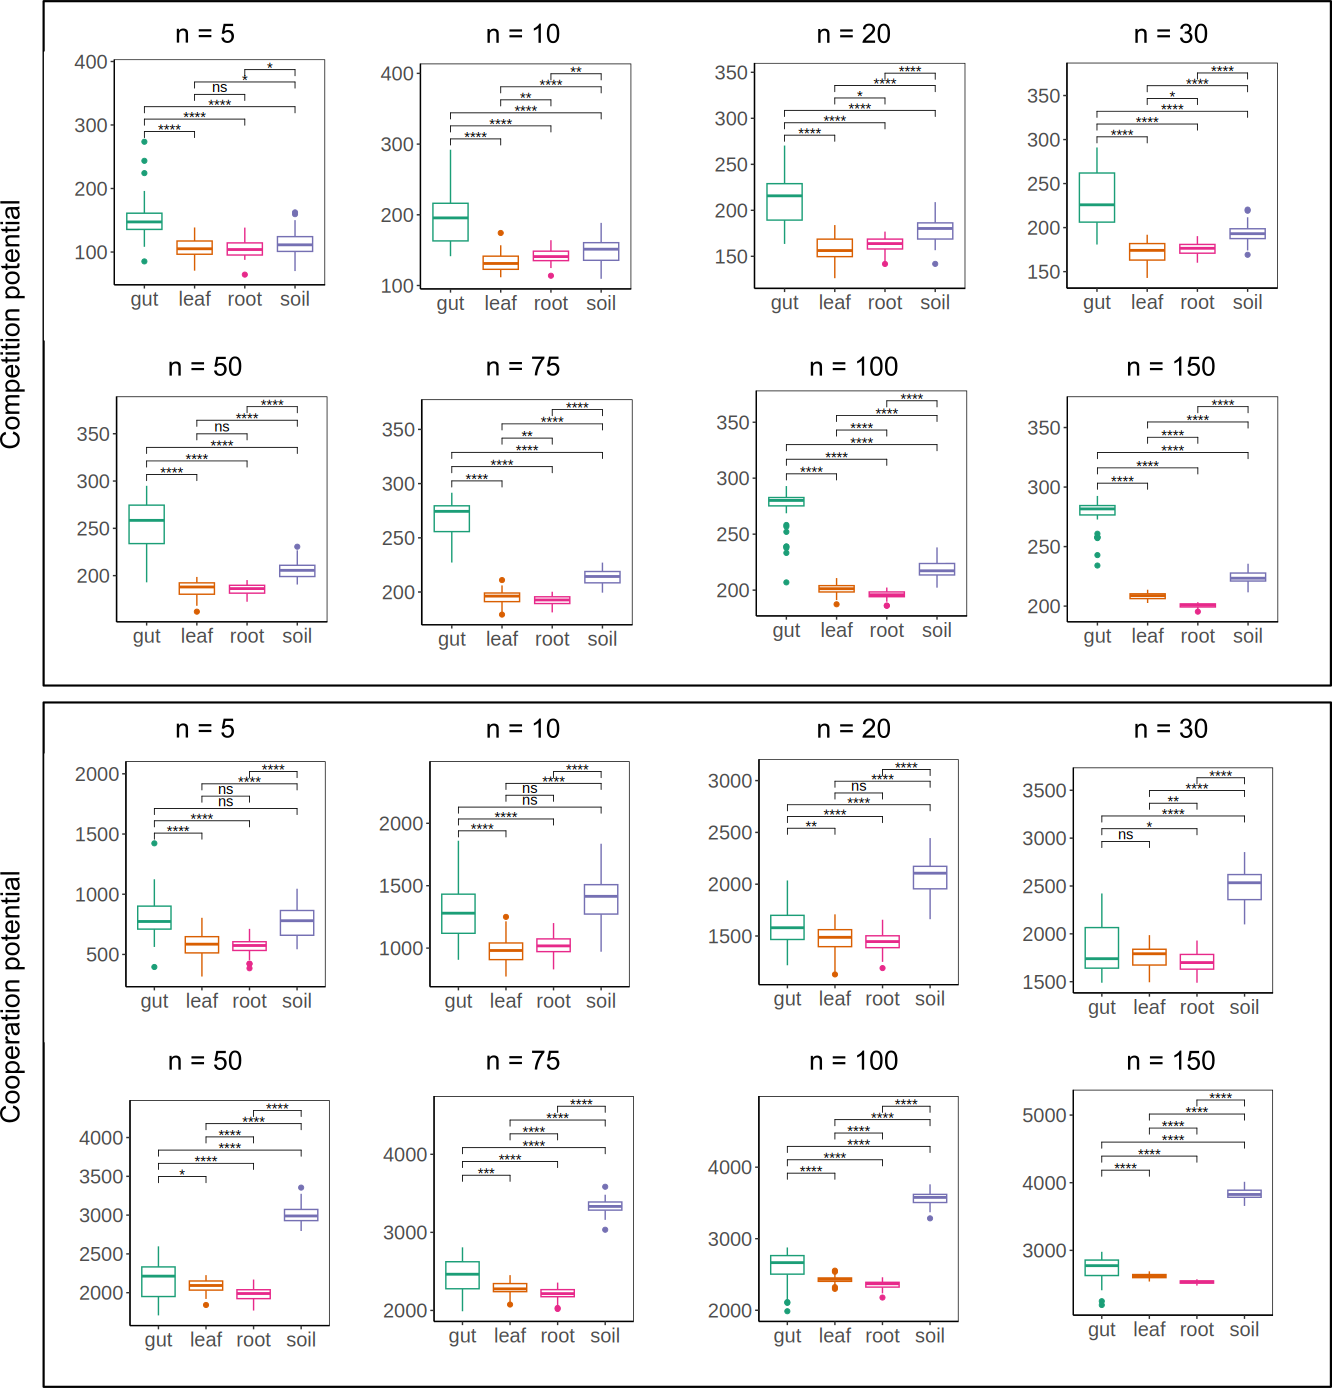
\includegraphics[width=0.8\textwidth]{img/annexe/ecosysteme_diff_potentials_specific.pdf}
    \caption{Distribution des scores de coopération et de compétition dans des communautés simulées de 5 à 150 bactéries isolé de l'intestin, de la racine , de la feuille et du sol en utilisant les graines spécifiques. Une comparaison de moyenne avec le test de Wilcoxon a été fait. }
    \label{fig:mix-diff-potentials}
\end{figure}

\newpage

\subsection*{Avec le mixte}

\begin{figure}[H]
    \centering
    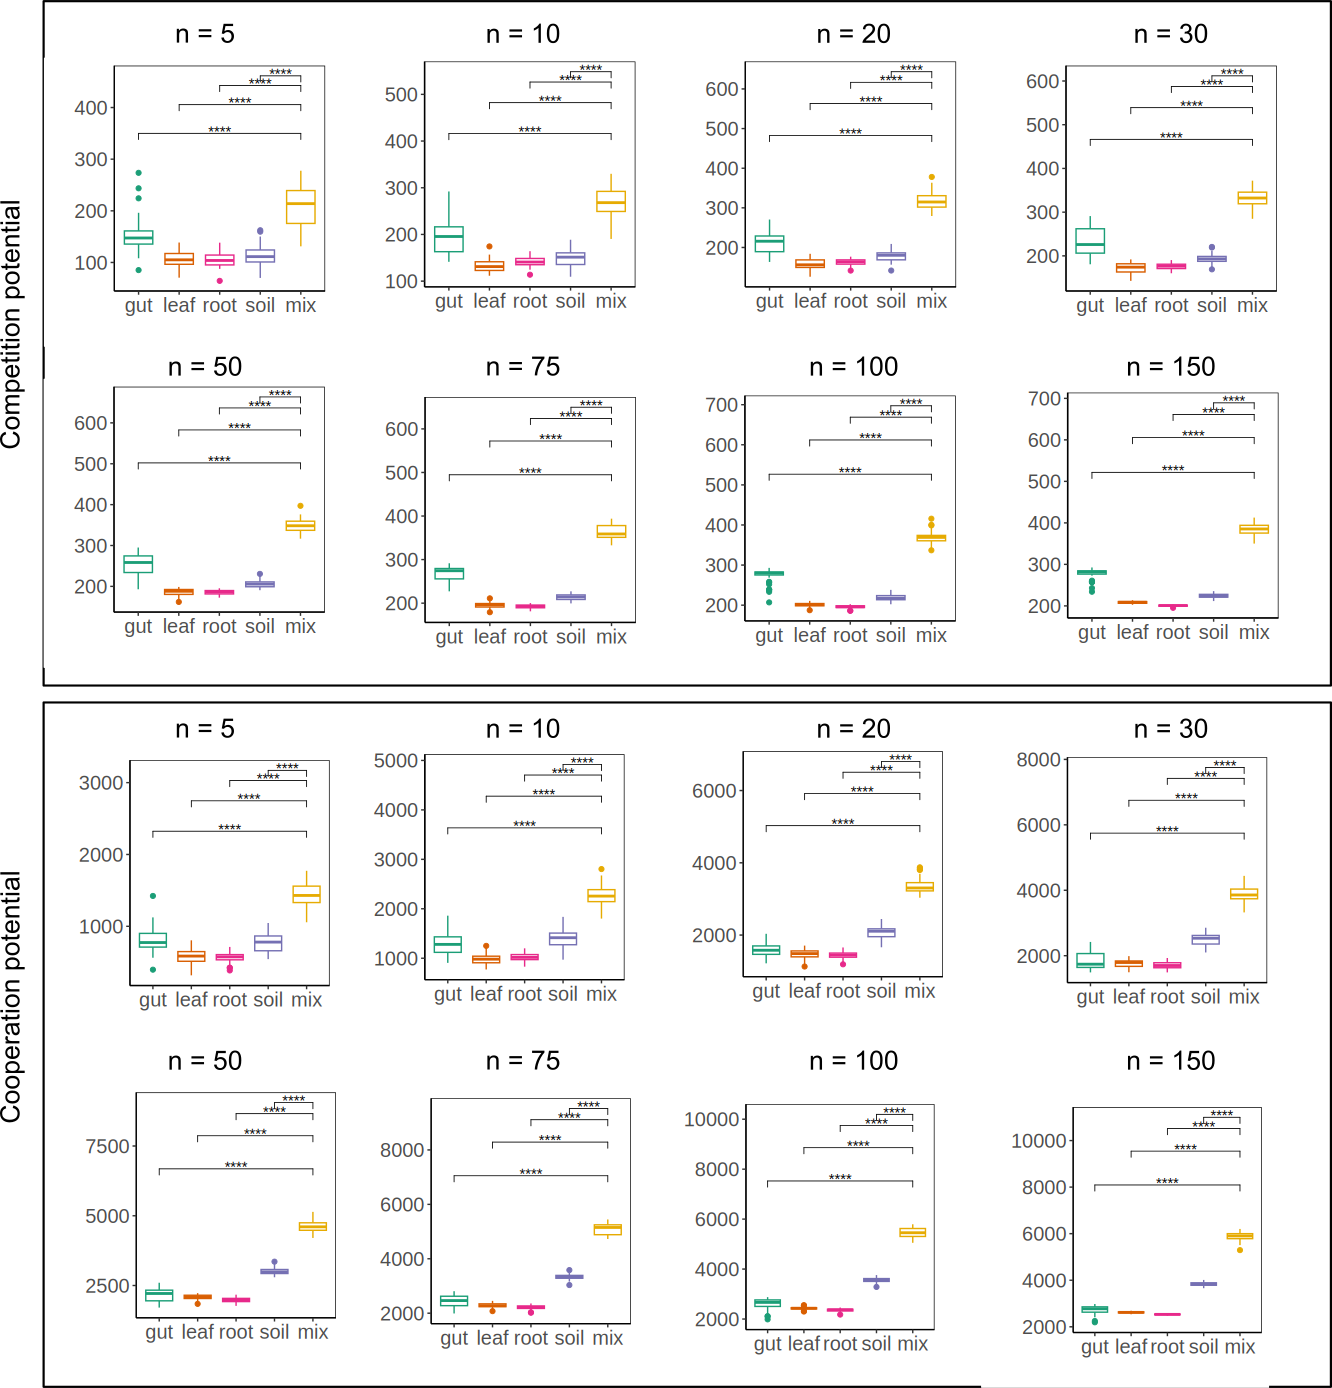
\includegraphics[width=0.8\textwidth]{img/annexe/mix_ecosysteme_diff_potentials_specific.pdf}
    \caption{Distribution des scores de coopération et de compétition dans des communautés simulées de 5 à 150 bactéries isolé de l'intestin, de la racine , de la feuille, sol et du mixte. Seul une comparaison avec deux à deux avec le mixte a été faite. La comparaison de moyenne avec le test de Wilcoxon a été fait. }
    \label{fig:mix-diff-potentials}
\end{figure}


\section*{Plus value d'ajout ou de retirer une espèces dans le milieu graine spécifique}
\addtocontents{toc}{\protect\contentsline {section}{B3 Plus value d'ajout ou de retirer une espèces dans le milieu graine spécifique}{}{}}
\begin{figure}[H]
    \centering
    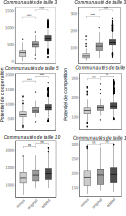
\includegraphics[width=0.7\textwidth]{img/annexe/added-value.pdf}
    \caption{Effet d'ajouter ("added") ou de retirer une espèce ("minus") sur les potentiels de coopération et de compétition pour chaque communauté acec les graines spécifiques. Le test de comparaison de moyenne Wilcoxon a été utilisé sur des communauté de taille 3 à 10 sur l'écosystème de l'intestin.}
    \label{fig:added-value}
\end{figure}


\section{Milieux générique et spécifique utilisés pour les simulations}
Les deux milieux spécifiques pour analyser le microbiote de l'intestin et ceux de la feuille, racine et du sol ainsi que le milieu générique sont représentés dans la Table \ref{graine-specific-generic}.

\newpage

\begin{table}[H]
\centering
\begin{adjustbox}{width=0.43\textwidth}
\begin{tabular}{|c|c|c|}
\hline
\begin{minipage}[t]{4cm}Composé du milieu générique\end{minipage}  & \begin{minipage}[t]{4cm}Composé du milieu spécifique pour la racine, feuille et le sol \end{minipage} & \begin{minipage}[t]{4cm}Composé du milieu spécifique pour l'intestin\end{minipage} \\
\hline
WATER&	WATER&	WATER \\
PROTON	&PROTON	&PROTON \\
CA+2	&CA+2	&CA+2 \\
K+	&K+	&K+ \\
MG+2	&MG+2	&MG+2 \\
NA+	&NA+&NA+ \\
Pi	&Pi	&Pi \\
CU+2&	CU+2	&CU+2 \\
FE+2&	FE+2	&FE+2 \\
FE+3&	FE+3	&FE+3 \\
MN+2	&MN+2	&MN+2 \\
ZN+2	&ZN+&2	ZN+2 \\
CL-	&CL-&	CL- \\
CPD-387	&CPD-387	&CPD-387 \\
AMMONIUM&	AMMONIUM&	AMMONIUM \\
NITRATE	&NITRATE	&NITRATE \\
OXYGEN-MOLECULE	&OXYGEN-MOLECULE	&OXYGEN-MOLECULE \\
SULFATE	&SULFATE	&SULFATE \\
SELENATE	&SELENATE	&SELENATE \\
ETOH	&MANNITOL	&ETOH \\
CELLULOSE	&GLC	&CELLULOSE \\
Starch&	L-CITRULLINE	&Starch \\
SORBITOL&	FRU	&SORBITOL \\
GLC	&FUM	&GLC \\
MANNITOL&	MAL	&MANNITOL \\
XYLITOL&	D-LACTATE	&XYLITOL \\
CPD-15972&	L-LACTATE&	CPD-15972 \\
MALTOSE&	METOH	&MALTOSE \\
SUCROSE&	SUC	&SUCROSE \\
D-galactopyranose&	SUCROSE	&D-galactopyranose \\
BETA-D-FRUCTOSE&	4-AMINO-BUTYRATE	&BETA-D-FRUCTOSE \\
DODECANOATE&	L-ALPHA-ALANINE	&DODECANOATE \\
PALMITATE	&ARG	&PALMITATE \\
STEARIC\_ACID	&ASN&	STEARIC\_ACID \\
OLEATE-CPD&	L-ASPARTATE	&OLEATE-CPD \\
ARACHIDIC\_ACID&	CYS&	ARACHIDIC\_ACID \\
ARACHIDONIC\_ACID	&GLN	&ARACHIDONIC\_ACID \\
BUTYRIC\_ACID&	GLT&	BUTYRIC\_ACID \\
CHOLESTEROL&	GLY	&CHOLESTEROL \\
TETRACOSANOATE&	HIS	&TETRACOSANOATE \\
LINOLEIC\_ACID	&ILE	&LINOLEIC\_ACID \\
ASCORBATE&	LEU	&ASCORBATE \\
PANTOTHENATE	&LYS&	PANTOTHENATE \\
DOCOSANOATE	& MET	&DOCOSANOATE \\
LINOLENIC\_ACID	&PHE&	LINOLENIC\_ACID \\
L-ALPHA-ALANINE&	PRO	&CPD-3617 \\
ASN	&SER	&CPD-7836 \\
ARG	&THR	&CPD-8462 \\
L-ASPARTATE&	TRP	&CPD-7830 \\
CYS	&TYR&	CPD-17322 \\
GLN	&VAL	&CPD-195 \\
GLT	&Vitamins-B12	&CPD-9245 \\
GLY&	COB-I-ALAMIN&	CPD-17188 \\
HIS	&CHOLINE&	CPD-13792 \\
ILE	&Reduced-ferredoxins	&CPD-12189 \\
LEU&	Acceptor	&CPD-12653 \\
LYS	& Donor-H2 	& CPD-14292 \\
MET	& ACP	& CPD0-2208 \\
PHE	& NAD	& CPD-10244 \\
PRO	 & NADP& 	L-ALPHA-ALANINE \\
SER	& ADP & 	ASN \\
THR	& &	ARG \\
TRP	& &	L-ASPARTATE \\
TYR	& &	CYS \\
VAL	& &	GLN \\
Vitamins-B12 & &		GLT \\
COB-I-ALAMIN	& &	GLY \\
CHOLINE	& &	HIS \\
THIAMINE	& &	ILE \\
ADENOSYLCOBALAMIN	& &	LEU \\
RIBOFLAVIN	& &	LYS \\
NIACINE	& &	MET \\
PYRIDOXAMINE	& &	PHE \\
PYRIDOXINE	& &	PRO \\
PYRIDOXAL	& &	SER \\
BIOTIN	& &	THR \\
VITAMIN\_D3	& &	TRP \\
ALPHA-TOCOPHEROL	& &	TYR \\
5-METHYL-THF	& &	VAL \\
THF	& &	Retinols \\
Acceptor	& &	THIAMINE \\
Donor-H2		& & ADENOSYLCOBALAMIN \\
Reduced-ferredoxins & &		RIBOFLAVIN \\
ACP	& &	NIACINE \\
NAD	& &	NIACINAMIDE \\
NADP	& &	PYRIDOXAMINE \\
ADP	& &	PYRIDOXINE \\
 &	&	PYRIDOXAL \\
	& &	BIOTIN \\
& &		VITAMIN\_D3 \\
	& &	ALPHA-TOCOPHEROL \\
& &		CPD-12826 \\
& &		10-FORMYL-THF \\
& &		5-METHYL-THF \\
& &		THF \\
& &		Vitamins-B12 \\
& &		COB-I-ALAMIN \\
& &		Acceptor \\
& &		Donor-H2 \\
& &		Reduced-ferredoxins \\
& &		ACP \\
& &		URATE \\
& &		CPD1F-129 \\
& &		NAD \\
& &		NADP \\
& & 	ADP \\
 \hline
\end{tabular}
\end{adjustbox}
\caption{\textbf{Composition du milieu générique et spécifique}}
\label{graine-specific-generic}
\end{table}

\chapter*{Contributions scientifiques}
\addtocontents{toc}{\protect\contentsline {chapter}{Annexe C Contributions scientifiques}{}{}}

\section*{Papier scientifique}
\addtocontents{toc}{\protect\contentsline {section}{C.1 Papier scientifique}{}{}}

\begin{itemize}
	\item \texttt{Article de journal}, Revealing the dynamics and mechanisms of bacterial interactions in cheese production with metabolic modelling, en révision\footnote{\url{https://www.sciencedirect.com/journal/metabolic-engineering}}, 2023
\end{itemize}

\section*{Posters}
\addtocontents{toc}{\protect\contentsline {section}{C.2 Poster}{}{}}

\begin{itemize}
	\item \texttt{Conférence nationale}, JOBIM conference, \textit{Journées Ouvertes en Biologie, Informatique et Mathématiques}, Characterising competition and cooperation potentials in microbial communities using discrete models of metabolism, 2022 
	\item \texttt{Conférence nationale}, JOBIM conference, \textit{Journées Ouvertes en Biologie, Informatique et Mathématiques}, Metabolic modelling deciphers interactions in a cheese bacterial community, 2021
	\item \texttt{conférence internationale}, MPA, \textit{Metabolic Pathway Analysis conference}, Metabolic modelling deciphers interactions in a cheese bacterial community, 2021
	\item \texttt{Conférence internationale}, CMSB \textit{19th International Conference on Computational Methods in Systems Biology}, Metabolic modelling deciphers interactions in a cheese bacterial community, 2021
\end{itemize}

\section*{Présentations orales}
\addtocontents{toc}{\protect\contentsline {section}{C.3 Présentations orales}{}{}}

\begin{itemize}
	\item \texttt{Séminaire} BioNum, \textit{Santé et bio-numérique}, Numerical and reasoning based metabolic modelling of bacterial communities, 2023
	\item \texttt{Conférence nationale}, Journée annuelle GT BIOSS, \textit{Groupe de travail sur la Biologie systémique symbolique}, Reasoning approaches for the characterization of cooperation and competition in large-scale microbial communities, 2022
	\item \texttt{Séminaire international}, GT SymBioDiversity, Characterizing microbial interactions in controlled and natural microbial communities \footnote{\url{https://eventos.cmm.uchile.cl/symbiodiversity/}}, 2022
	\item \texttt{Conférence nationale} METABODAY, Metabolic modelling deciphers interactions in a cheese bacterial community, 2021
\end{itemize} 









\end{document}